\documentclass[a4paper, 14pt]{extarticle}

\usepackage[T2A]{fontenc}
\usepackage{natbib}
\usepackage{graphicx}
\usepackage[english, russian]{babel}
\usepackage{fontspec}
\usepackage{amsmath}
\usepackage{amsfonts}
\usepackage{amssymb}
\usepackage{amsthm}
\usepackage{mathtools}
\usepackage{mathrsfs}
\usepackage{icomma}
\usepackage{fullpage}
\usepackage{ulem}
\usepackage{setspace}
\usepackage{listings}
\usepackage{indentfirst}
\usepackage[left=2cm,right=1.5cm,top=2cm,bottom=2cm]{geometry}
\usepackage{xcolor}
\usepackage{float}
\usepackage{csquotes}
\usepackage{hyperref}
\usepackage{graphics}
\usepackage{wasysym}
\usepackage{titlesec}



\definecolor{urlcolor}{HTML}{0000FF} % цвет гиперссылок
\definecolor{linkcolor}{HTML}{000000} % цвет гиперссылок
\hypersetup{pdfstartview=FitH, linkcolor=linkcolor, urlcolor=urlcolor, colorlinks=true}


\setmainfont{Times New Roman}
\setlength{\parindent}{5ex}
\setlength{\parskip}{1em}
\renewcommand{\baselinestretch}{1}

\graphicspath{{images/}}


\definecolor{buzzlightyear}{HTML}{8757A5}
\definecolor{grass}{HTML}{738D06}
\definecolor{literal}{HTML}{F18A2B}
\definecolor{commentcolor}{HTML}{8E908B}

\lstdefinestyle{habrstyle}{
    backgroundcolor=\color{white},
    commentstyle=\color{commentcolor},
    keywordstyle=\bfseries\color{buzzlightyear},
    numberstyle=\tiny\color{commentcolor},
    stringstyle=\color{grass},
    basicstyle=\ttfamily\footnotesize,
    breakatwhitespace=false,
    breaklines=true,
    captionpos=b,
    keepspaces=true,
    numbers=left,
    numbersep=5pt,
    showspaces=false,
    showstringspaces=false,
    showtabs=false,
    tabsize=4
}

\lstset{style=habrstyle}

\begin{document}
    % НАЧАЛО ТИТУЛЬНОГО ЛИСТА
    \begin{center}
        \begin{center}
            \hfill \break
            \normalsize{Санкт-Петербургский государственный политехнический}\\
            \normalsize{университет Петра Великого}\\
            \hfill \break
            \normalsize{\textbf{Высшая школа интеллектуальных систем и}}\\
            \normalsize{\textbf{суперкомпьютерных технологий}}\\
            \hfill \break
            \hfill \break
            \hfill \break
            \normalsize{Лабораторная работа}\\
            \hfill \break
            \normalsize{\LARGE GNU Radio}\\
        \end{center}
        \hfill \break
        \hfill \break
        \hfill \break
        \hfill \break
        \hfill \break
        \hfill \break
        \hfill \break
        \hfill \break
        \hfill \break
        \hfill \break
        \begin{tabbing}
            Выполнил студент гр. 3530901/80201 \`И.С. Иванов\\
            \\
            Преподаватель: \`Н.В. Богач\\
        \end{tabbing}
        \hfill \break
        \hfill \break
        \hfill \break
        \hfill \break
        \begin{center}
            Санкт-Петербург\\
            2021
        \end{center}
        \thispagestyle{empty}
    \end{center}
    % КОНЕЦ ТИТУЛЬНОГО ЛИСТА

    % ОГЛАВЛЕНИЕ
    \newpage
    \tableofcontents

    % СПИСОК ИЛЛЮСТРАЦИЙ
    \newpage
    \listoffigures

    \newpage


    \section{Передача сигнала}
    \label{sec:1}

    Первый этап - передача сигнала QPSK.
    Необходимо сгенерировать поток битов и смоделировать его на сложное созвездие.
    Для этого мы используем блок \texttt{Constellation Modulator}.

    Объект созвездия позволяет нам определить, как кодируются символы.
    Затем блок модулятора может использовать эту схему модуляции с дифференциальным кодированием или без него.
    Модулятор созвездия ожидает упакованные байты, поэтому у нас есть генератор случайного источника, предоставляющий байты со значениями 0-255.

    Количество выборок на символ должно быть минимальным для обеспечения желаемой скорости передачи данных.
    Мы будем использовать 4, что больше, чем нам нужно.
    Это необходимо для лучшей визуализации сигнала в различных областях.

    Наконец, мы устанавливаем значение избыточной пропускной способности.
    Посмотрим на полученный \texttt{flowgraph}.

    \begin{figure}[H]
        \centering
        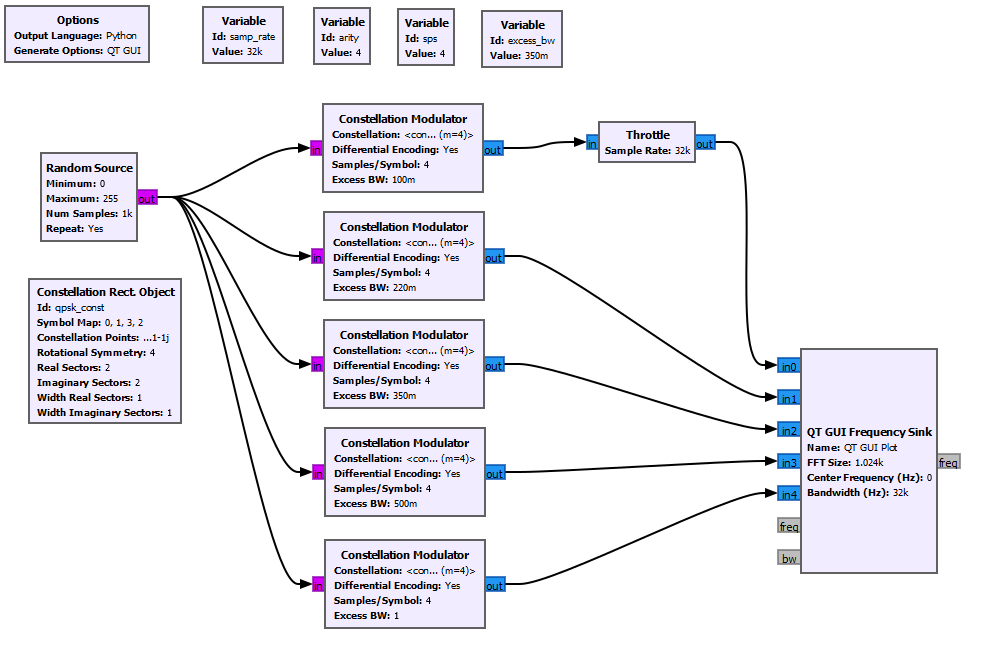
\includegraphics[width=0.8\linewidth]{flowgraph}
        \caption{Flowgraph избыточной пропускной способности}
        \label{fig:flowgraph}
    \end{figure}

    После запуска получаем график, показывающий различные значения избыточной пропускной способности.
    Типичные значения находятся в диапазоне от 0,2 (красная кривая) до 0,35 (зеленая кривая).

    \begin{figure}[H]
        \centering
        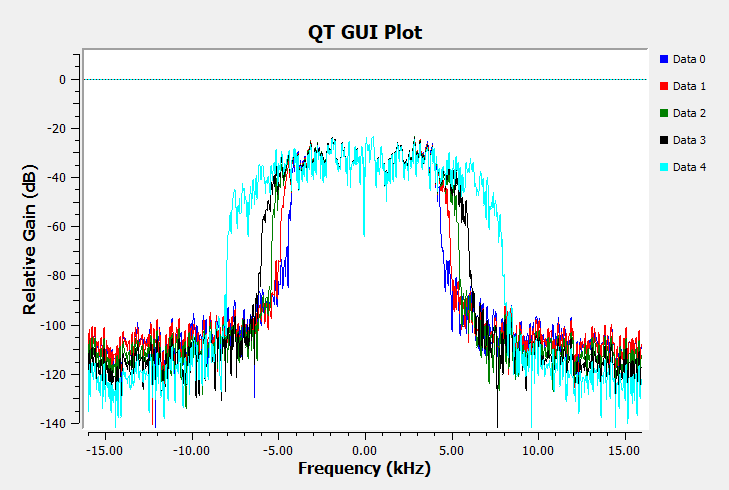
\includegraphics[width=0.8\linewidth]{flowgraph_wave}
        \caption{Избыточная пропускная способность}
        \label{fig:flowgraph_wave}
    \end{figure}

    Далее запустим файл \texttt{mpsk\_stage1.grc}, передающий созвездие QPSK.

    \begin{figure}[H]
        \centering
        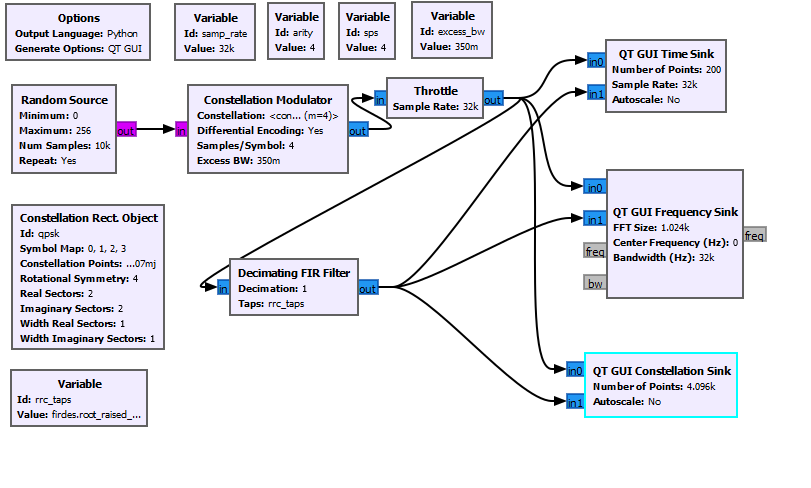
\includegraphics[width=0.8\linewidth]{flowgraps_qpsk_constellation}
        \caption{Flowgraph созвездия QPSK}
        \label{fig:flowgraps_qpsk_constellation}
    \end{figure}

    \begin{figure}[H]
        \centering
        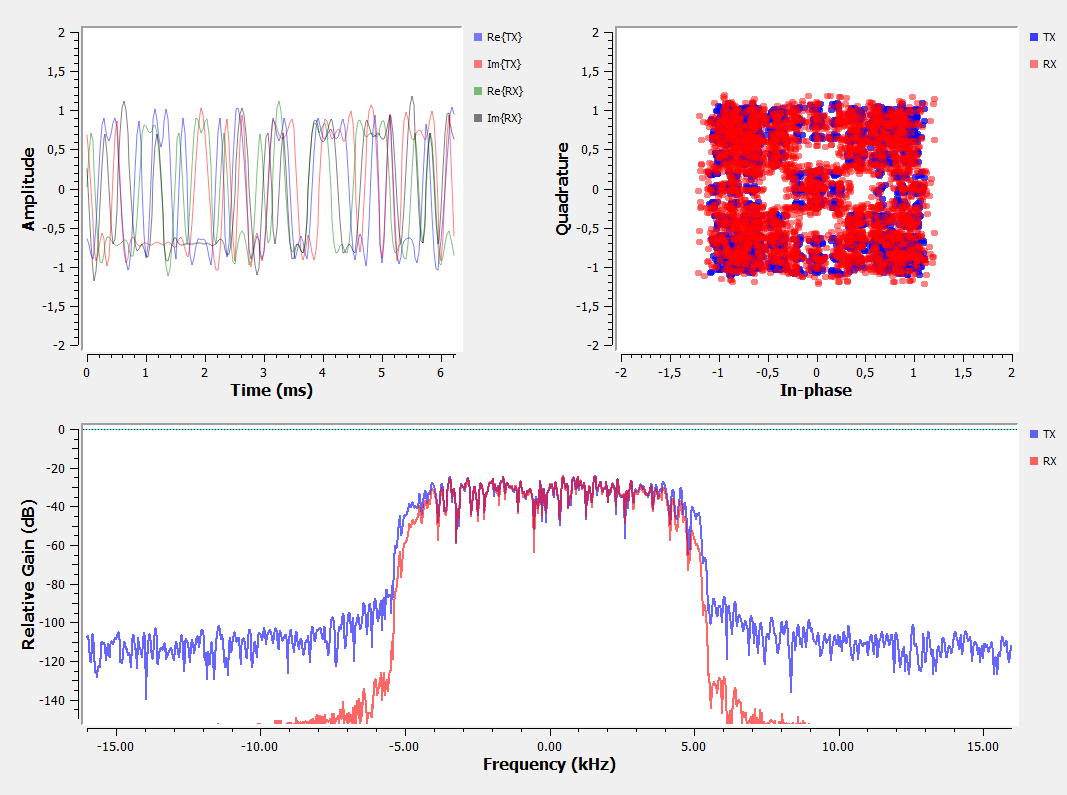
\includegraphics[width=0.8\linewidth]{qpsk_constellation}
        \caption{Созвездие QPSK}
        \label{fig:qpsk_constellation}
    \end{figure}

    На графике созвездия мы видим эффекты повышающей дискретизации и процесс фильтрации.
    В этом случае фильтр RRC добавляет преднамеренные самоинтерференции(ISI).

    На стороне приема мы избавляемся от ISI с помощью другого фильтра RRC.
    В результате, мы сворачиваем два фильтра RRC вместе, и получаем фильтр с приподнятым косинусом.

    Фильтрация представляет собой просто свертку, поэтому выходной сигнал RRC-фильтра на приемной стороне представляет собой сигнал в форме приподнятого косинусоидального импульса с минимизированным ISI.
    Другое преимущество состоит в том, что при отсутствии эффектов канала мы используем согласованный фильтр на приемнике.

    \newpage


    \section{Добавление нарушений канала}
    \label{sec:2}

    Теперь мы рассмотрим влияние канала на то, как сигнал искажается между передачей и приёмом.
    Для начала мы будем использовать самый простой блок модели канала GNU Radio, который позволит нам смоделировать несколько основных проблем связанных с приёмником.

    Проблемы:
    \begin{enumerate}
        \item Шум.
        В нашем приемнике вызывается аддитивный белый гауссовский шум. Мы устанавливаем мощность этого шума, регулируя значение напряжения шума модели канала.
        \item \texttt{clock}, определяющие частоту радиомодулей.
        Два радиомодуля имеют разные \texttt{clock}. Одно радио работает на частоте \texttt{fc + f\_delta\_1}.
        Другое радио имеет другие \texttt{clock} и его реальная частота равна \texttt{fc + f\_delta\_2}.
        \item Таким образом, полученный сигнал будет \texttt{f\_delta\_1 + f\_delta\_2}.
        \item Идеальная точка выборки.
        Идеальная точка выборки связана с проблемой часов.
        Два радиомодуля работают с разной скоростью, поэтому идеальная точка выборки неизвестна.
    \end{enumerate}

    Результат моделирования позволяет нам поработать с аддитивным шумом, сдвигом частоты и временным сдвигом.

    \begin{figure}[H]
        \centering
        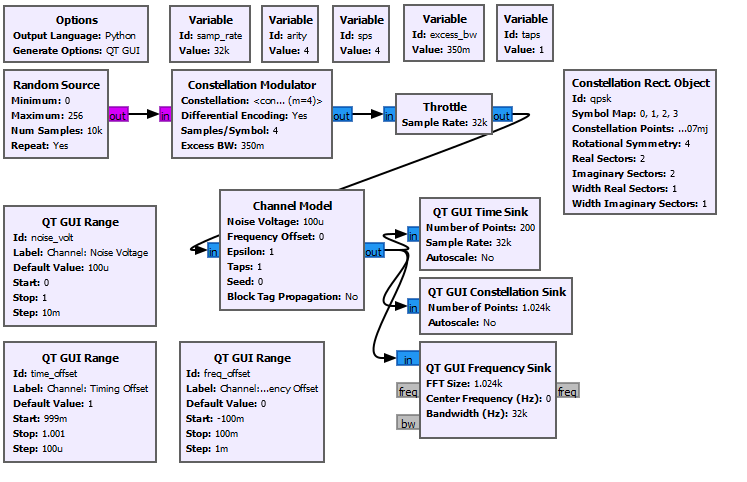
\includegraphics[width=0.8\linewidth]{flowgraph_channel_impairments}
        \caption{Flowgraph с добавлением нарушения канала}
        \label{fig:flowgraph_channel_impairments}
    \end{figure}

    \begin{figure}[H]
        \centering
        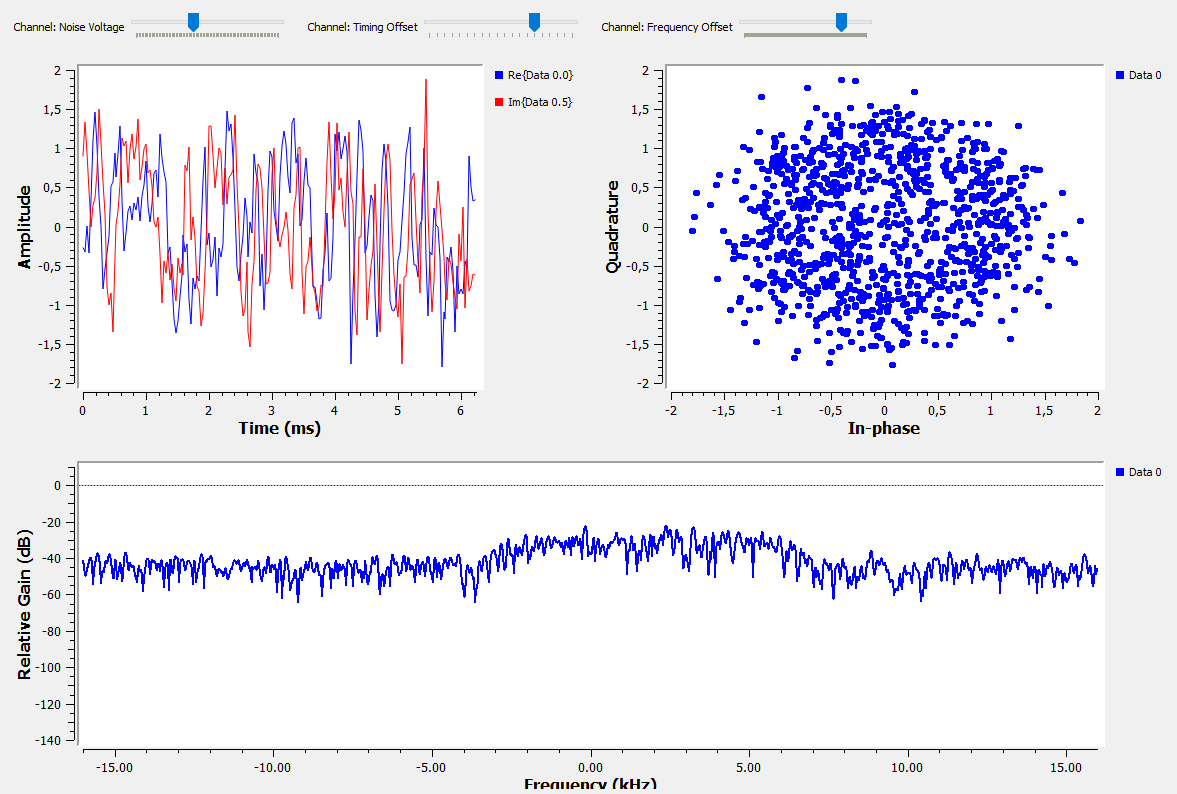
\includegraphics[width=0.8\linewidth]{channel_impairments}
        \caption{Добавление нарушения канала}
        \label{fig:channel_impairments}
    \end{figure}

    График созвездия показывает нам облако образцов, намного хуже того, с чего мы начали на последнем этапе.
    Теперь, исходя из полученного сигнала, мы должны отменить все эти эффекты.

    \newpage


    \section{Восстановление \texttt{timing}}
    \label{sec:3}

    Теперь перейдём к процессу восстановления.
    Здесь мы будем использовать алгоритм восстановления многофазных \texttt{clocks}.
    Мы начнем с восстановления \texttt{timing}.
    Мы пытаемся найти наилучшее время для дискретизации входящих сигналов, что позволит максимизировать отношение сигнал/шум (SNR) каждой выборки, а также уменьшить влияние межсимвольных помех (ISI).

    \subsection{ISI}

    Проблему ISI мы можем увидеть на примере flowgraph \texttt{symbol\_sampling.grc}, где мы создаем четыре отдельных символа, а затем фильтруем их.

    \begin{figure}[H]
        \centering
        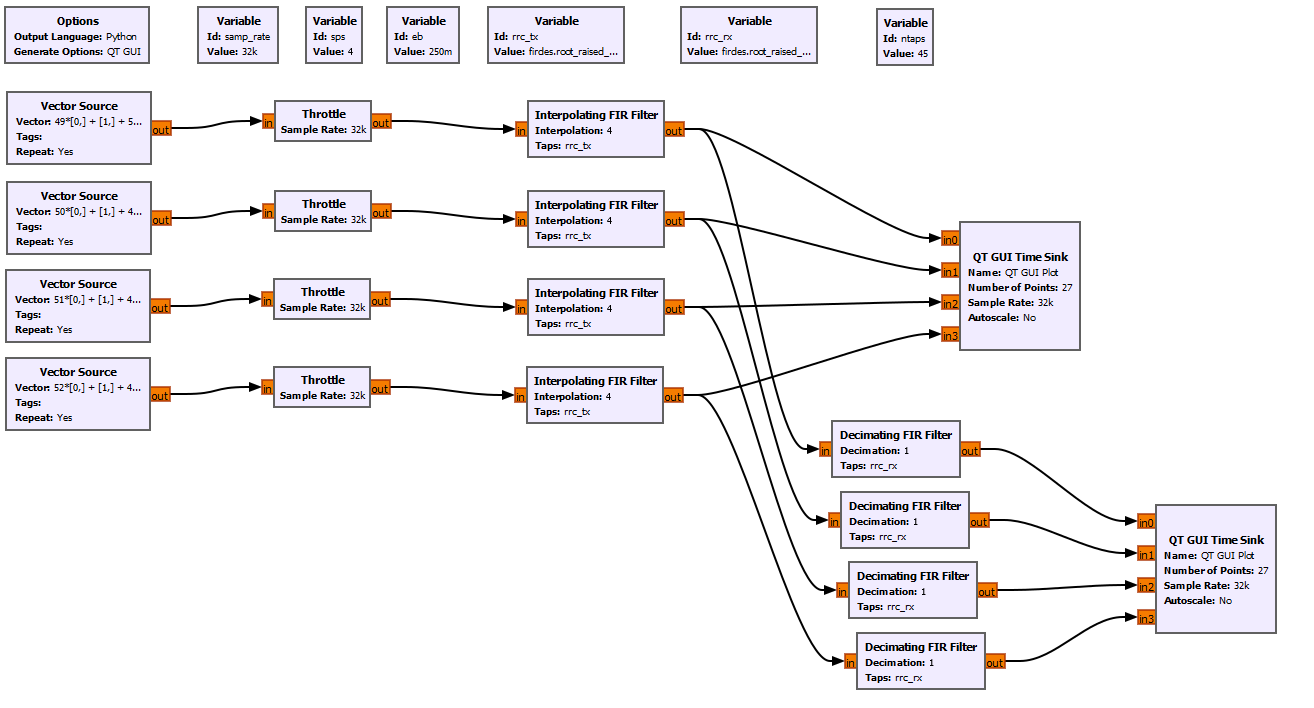
\includegraphics[width=0.8\linewidth]{flowgraph_isi_problem}
        \caption{Flowgraph проблемы ISI}
        \label{fig:flowgraph_isi_problem}
    \end{figure}

    \begin{figure}[H]
        \centering
        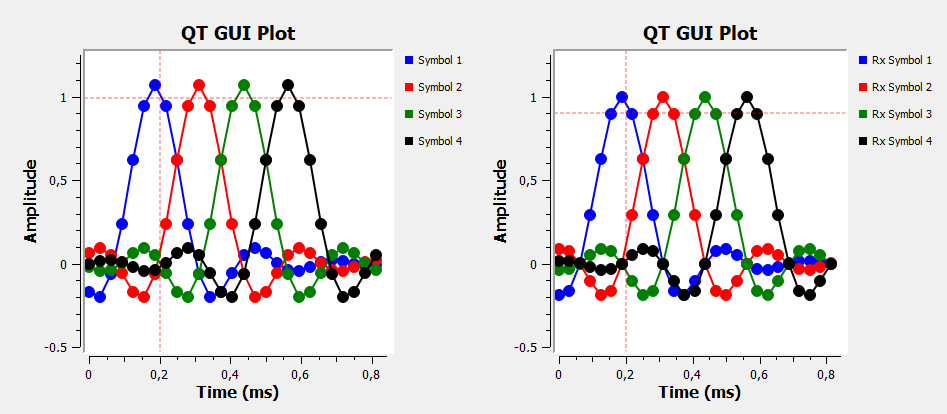
\includegraphics[width=0.8\linewidth]{isi_problem}
        \caption{Передача 4-ех символов без рассинхронизации}
        \label{fig:isi_problem}
    \end{figure}

    На графике видны различия между символами, отфильтрованными RC и RRC.
    Без фильтрации Найквиста (RRC - справа) мы можем увидеть, как в идеальной точке выборки каждого символа другие символы имеют некоторую энергию.
    Если мы суммируем эти символы вместе (как в непрерывном потоке), то энергия других выборок складывается вместе и искажает символ в этой точке.
    И наоборот, на выходе с RC-фильтром энергия от других выборок равна 0 в идеальной точке дискретизации для данного символа во времени.
    Это означает, что если мы делаем выборку точно в правильной точке выборки, мы получаем энергию только от текущего символа без помех от других символов в потоке.
    Это моделирование позволяет нам легко настроить количество выборок на символ, избыточную полосу пропускания фильтров RRC и количество ответвлений.

    \subsection{Разные \texttt{clocks}}

    Затем мы посмотрим, как разные часы влияют на точки выборки между передатчиком и приемником.
    Используя пример потокового графа в \texttt{symbol\_sampling\_diff.grc}, мы моделируем влияние разных часов в передатчике и приемнике.

    \begin{figure}[H]
        \centering
        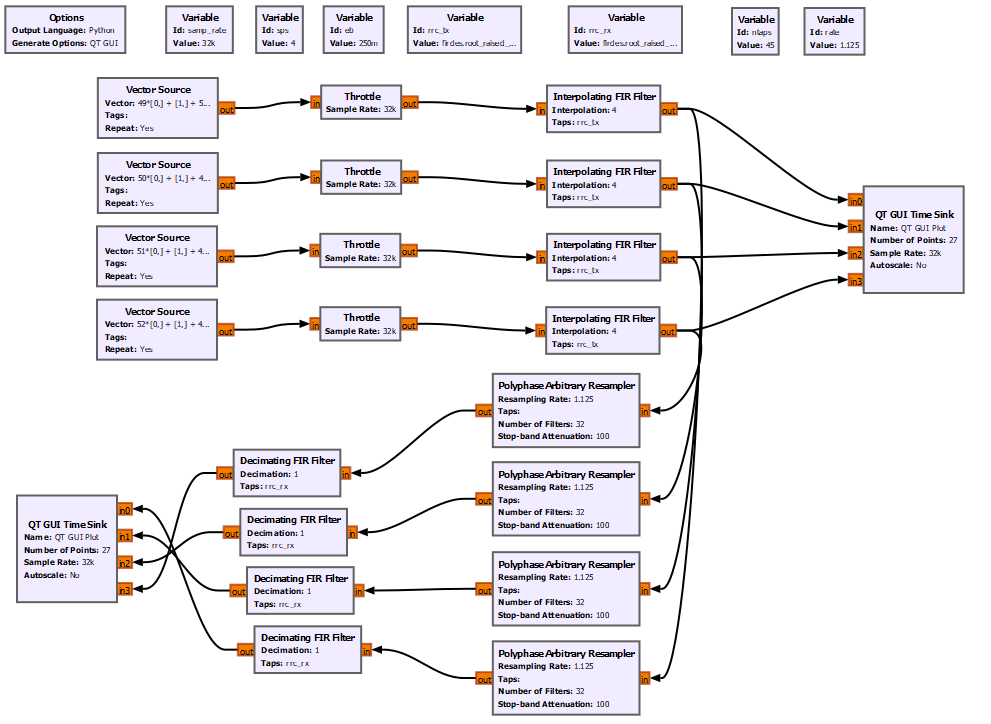
\includegraphics[width=0.8\linewidth]{flowgraph_diff_clocks}
        \caption{Flowgraph разные clocks}
        \label{fig:flowgraph_diff_clocks}
    \end{figure}

    Все часы несовершенные, поэтому они:
    \begin{enumerate}
        \item начнут свою работу в разные моменты времени;
        \item дрейфуют относительно других часов.
    \end{enumerate}

    \begin{figure}[H]
        \centering
        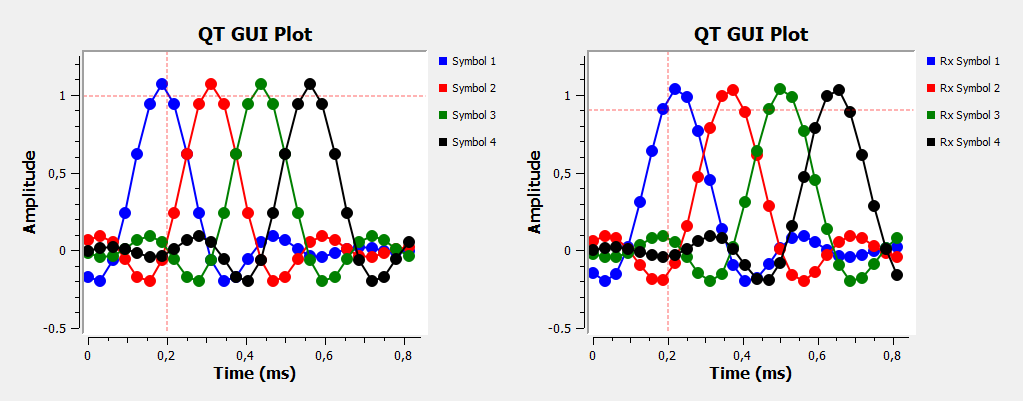
\includegraphics[width=0.8\linewidth]{diff_clocks}
        \caption{Передача 4-ех символов с рассинхронизации}
        \label{fig:diff_clocks}
    \end{figure}

    Наша задача - синхронизировать часы передачи и приемника, используя только информацию в приемнике из входящих выборок.
    Это задача известна как восстановление часов или времени.

    \subsection{Блок синхронизации многофазных часов}

    Блок вычисляет первый дифференциал входящего сигнала, который будет связан с его смещением тактовой частоты.
    В примере flowgraph \texttt{symbol\_differential\_filter.grc}, можно увидеть графики с параметром скорости 1 (т.е. нет смещения часов).

    Нам нужен образец 0,22 мс. Фильтр разности ([-1, 0, 1]) генерирует дифференциал символа, и выходной сигнал этого фильтра в правильной точке выборки равен 0.
    Затем мы можем инвертировать этот оператор и вместо этого сказать, когда выход дифференциального фильтра равен 0, мы нашли оптимальную точку выборки.

    \begin{figure}[H]
        \centering
        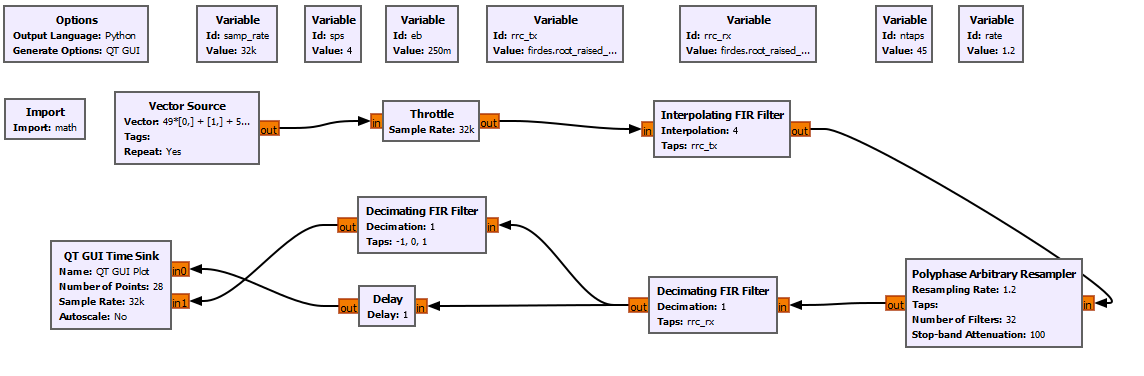
\includegraphics[width=0.8\linewidth]{flowgraph_diff_filter}
        \caption{Применение функции sample}
        \label{fig:flowgraph_diff_filter}
    \end{figure}

    \begin{figure}[H]
        \centering
        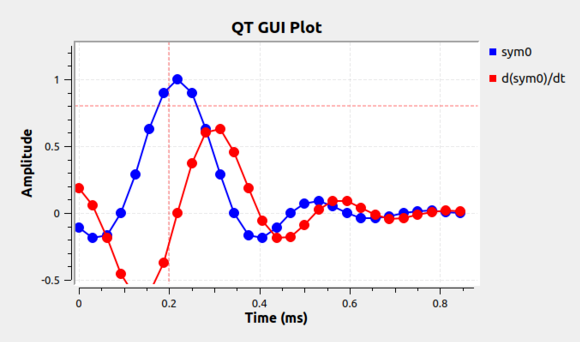
\includegraphics[width=0.8\linewidth]{diff_filter_without}
        \caption{Нет смещения часов}
        \label{fig:diff_filter_without}
    \end{figure}

    У нас есть временное смещение там, где пик символа выключен, а производный фильтр не показывает нам нулевую точку.

    \begin{figure}[H]
        \centering
        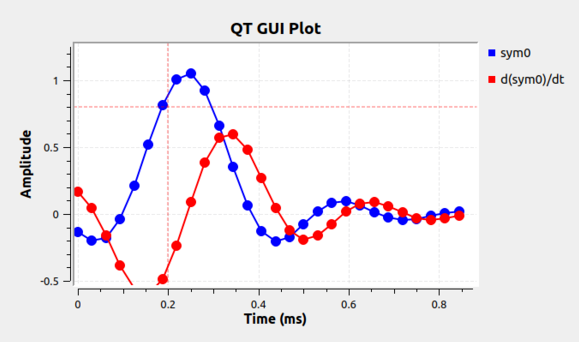
\includegraphics[width=0.8\linewidth]{diff_filter_with}
        \caption{Есть смещение часов}
        \label{fig:diff_filter_with}
    \end{figure}

    Вместо использования одного фильтра мы можем создать серию фильтров, каждый с разной фазой.
    Если у нас достаточно фильтров на разных фазах, один из них имеет правильную фазу фильтра, которая даст нам желаемое значение синхронизации.
    Посмотрим на симуляцию, которая строит 5 фильтров, что означает 5 различных фаз.

    \begin{figure}[H]
        \centering
        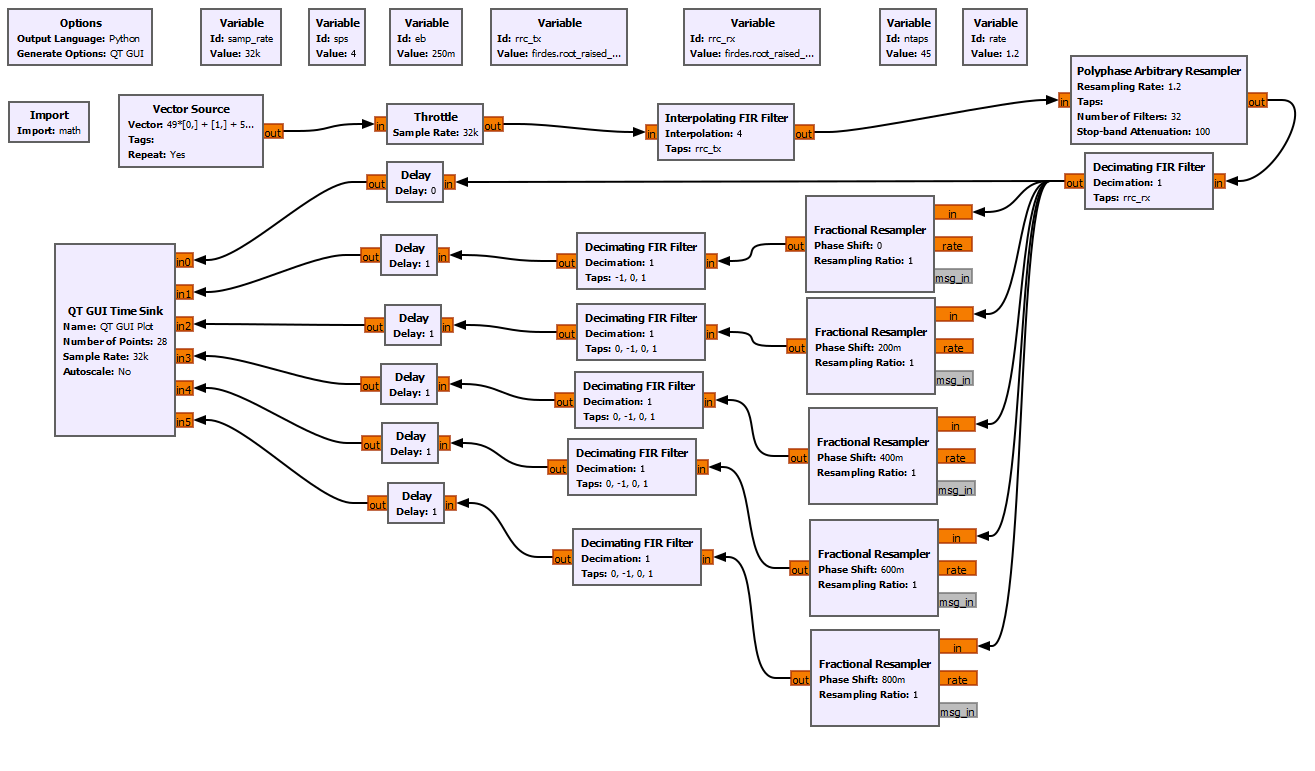
\includegraphics[width=0.8\linewidth]{flowgraph_filter_diff_phase}
        \caption{Flowgraph с несколькими фазами}
        \label{fig:flowgraph_filter_diff_phase}
    \end{figure}

    \begin{figure}[H]
        \centering
        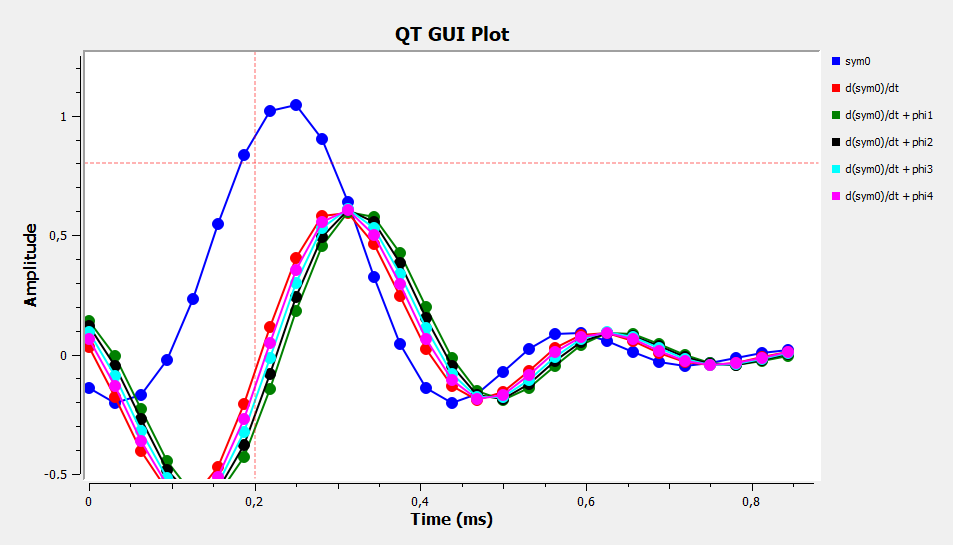
\includegraphics[width=0.8\linewidth]{diff_filter_phase}
        \caption{Несколько фаз}
        \label{fig:filter_diff_filter_phase}
    \end{figure}

    На графике мы можем видеть, что сигнал, помеченный как $d(sym0)/dt+phi3$, имеет точку отсчета в 0.
    Это говорит нам о том, что наша идеальная точка дискретизации находится при этом фазовом сдвиге.
    Следовательно, если мы возьмем RRC-фильтр нашего приемника и настроим его фазу на $phi3=3*2\pi/5$, то мы сможем исправить рассогласование по времени и выбрать идеальную точку дискретизации.

    Итак, в данном примере мы использовали 5 фильтров в качестве идеальной точки выборки.
    Но этого недостаточно.
    Любое смещение выборки между этими фазами по-прежнему приведет к несвоевременной выборке с добавленными ISI, как мы исследовали ранее.

    Поэтому мы используем больше фильтров (32), чтобы получить максимальный коэффициент шума ISI, который меньше шума квантования 16-битного значения.
    То есть мы получим точность 16 бит. Для большей точность потребуется больше фильтров.

    Затем мы используем контур управления 2-го порядка, который требуется, чтобы получить как правильную фазу фильтра, так и разницу в скорости между двумя тактовыми сигналами.

    \subsection{Использование блока многофазной синхронизации}

    Теперь мы используем этот блок в нашей симуляции.
    Пример flowgraph \texttt{mpsk\_stage3.grc} принимает выходные данные модели канала и передает их через наш блок.

    \begin{figure}[H]
        \centering
        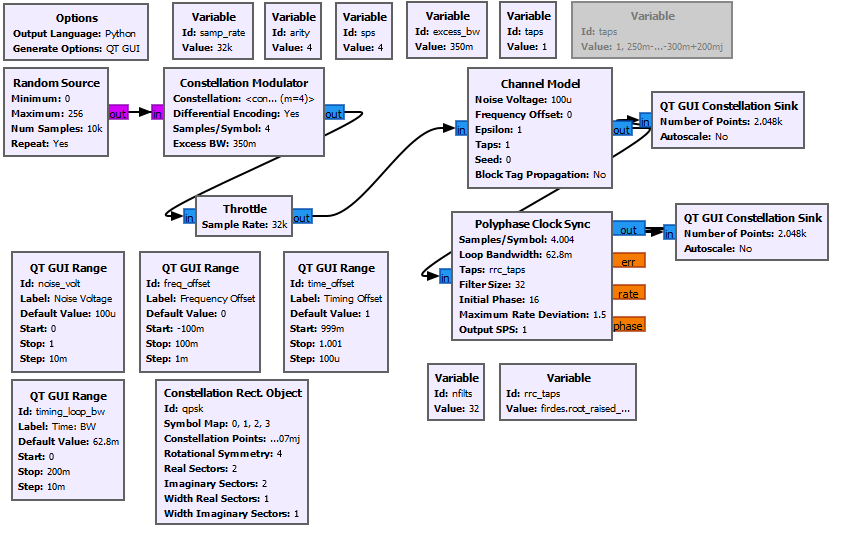
\includegraphics[width=0.8\linewidth]{flowgraph_multyphase}
        \caption{Flowgraph с блоком многофазной синхронизации}
        \label{fig:flowgraph_multyphase}
    \end{figure}

    \begin{figure}[H]
        \centering
        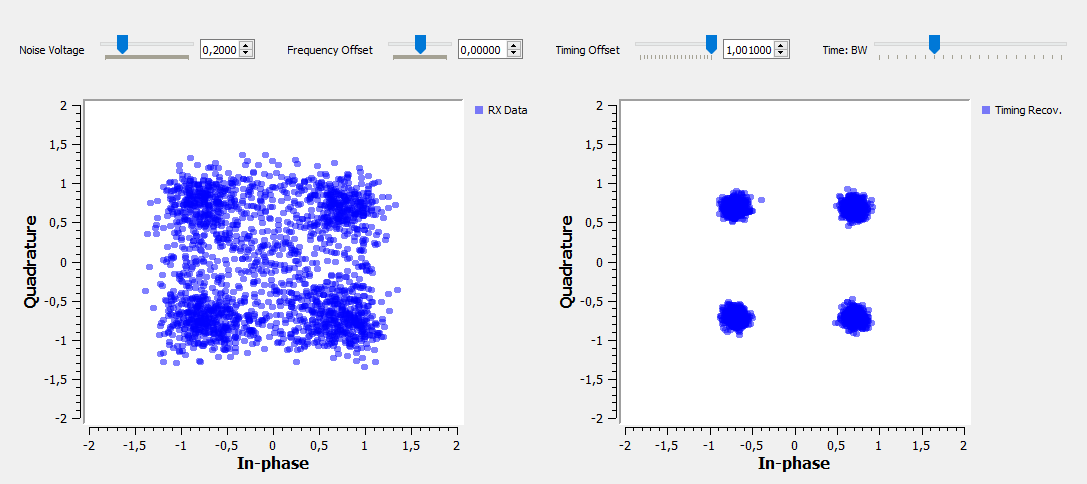
\includegraphics[width=0.8\linewidth]{multiphase}
        \caption{Использование блока многофазной синхронизации}
        \label{fig:multiphase}
    \end{figure}

    Видно два созвездия: слева - полученный сигнал до восстановления синхронизации и справа - после восстановления синхронизации.

    \newpage


    \section{Многолучевость}
    \label{sec:4}

    Сначала мы разберемся, что такое многолучевость.
    В большинстве коммуникационных сред у нас нет единственного пути для прохождения сигнала от передатчика к приемнику.
    Сигналы отражаются от различных поверхностей и приходят на приёмник в разное время в зависимости от длины пути.
    Их суммирование в приемнике вызывает искажения.
    Эти искажения вызывают внутрисимвольную и межсимвольную интерференции.

    Нам нужно исправить это поведение, и мы можем сделать это, используя механизм, очень похожий на стереоэквалайзер.
    С помощью стереофонического эквалайзера мы можем изменить усиление определенных частот, чтобы либо подавить, либо усилить эти сигналы.

    \begin{figure}[H]
        \centering
        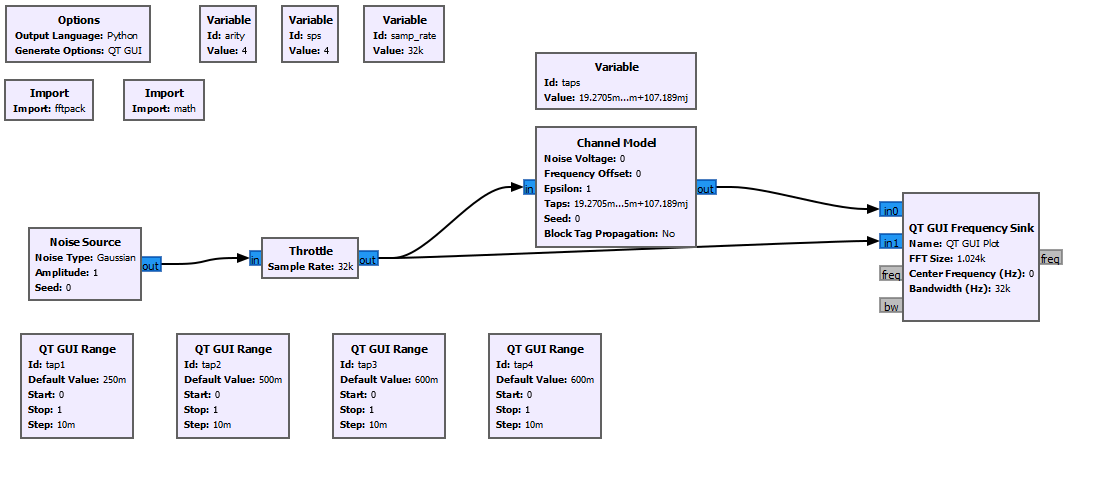
\includegraphics[width=0.8\linewidth]{flowgraph_multipath_sim}
        \caption{Flowgraph многолучевость}
        \label{fig:flowgraph_multipath_sim}
    \end{figure}

    \begin{figure}[H]
        \centering
        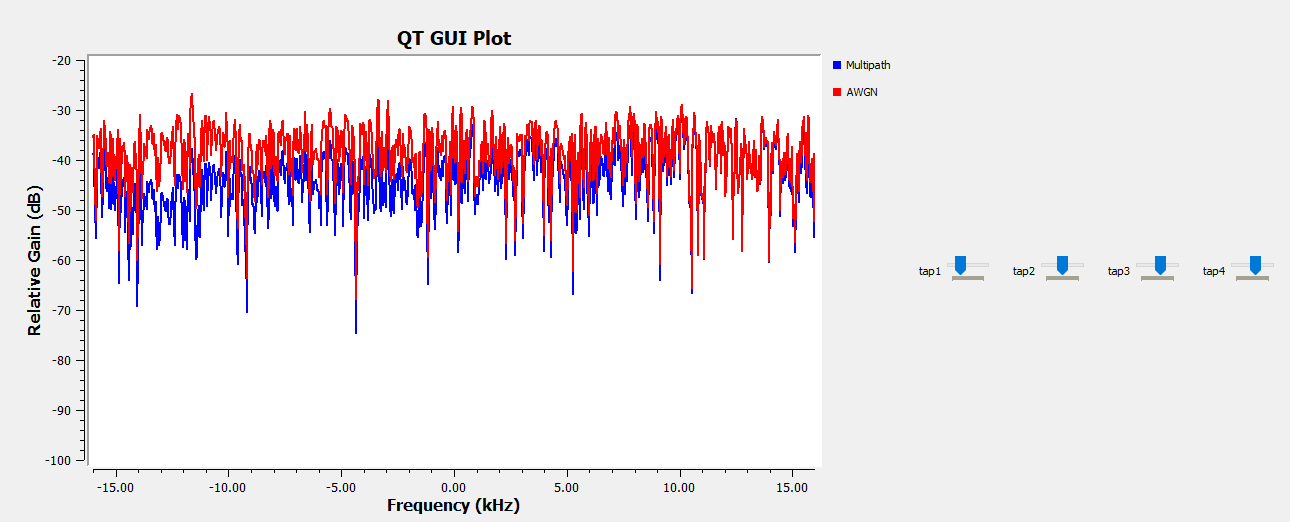
\includegraphics[width=0.8\linewidth]{multipath_sim}
        \caption{Использование блока многофазной синхронизации}
        \label{fig:multipath_sim}
    \end{figure}

    Как мы можем видеть на графике, многолучевой канал создает некоторые искажения в сигнале.
    Задача эквалайзера - отменить искажение, вызванное каналом, чтобы выходной сигнал эквалайзера был ровным.
    Но вместо того, чтобы настраивать каждый tap вручную, мы используем алгоритмы, которые обновляют эти taps за нас.
    Наша задача - использовать правильный алгоритм эквалайзера и настроить параметры.

    Одним из важных параметров здесь является количество taps в эквалайзере.
    Как мы видим в нашем моделировании, пять taps дают довольно грубый контроль над частотной характеристикой.
    Чем больше taps, тем больше времени требуется как на вычисление ответвлений, так и на запуск эквалайзера против сигнала.

    \newpage


    \section{Эквалайзеры}
    \label{sec:5}

    GNU Radio имеет два эквалайзера.

    \subsection{CMA}

    CMA или алгоритм постоянного модуля - это слепой эквалайзер, который работает только с сигналами с постоянной амплитудой или модулем.
    В примере \texttt{mpsk\_stage4.grc} мы используем алгоритм CMA с 11 taps.
    Изменим параметры и посмотрим, как это влияет на производительность как с точки зрения вычислений, так и с точки зрения сигналов.

    \begin{figure}[H]
        \centering
        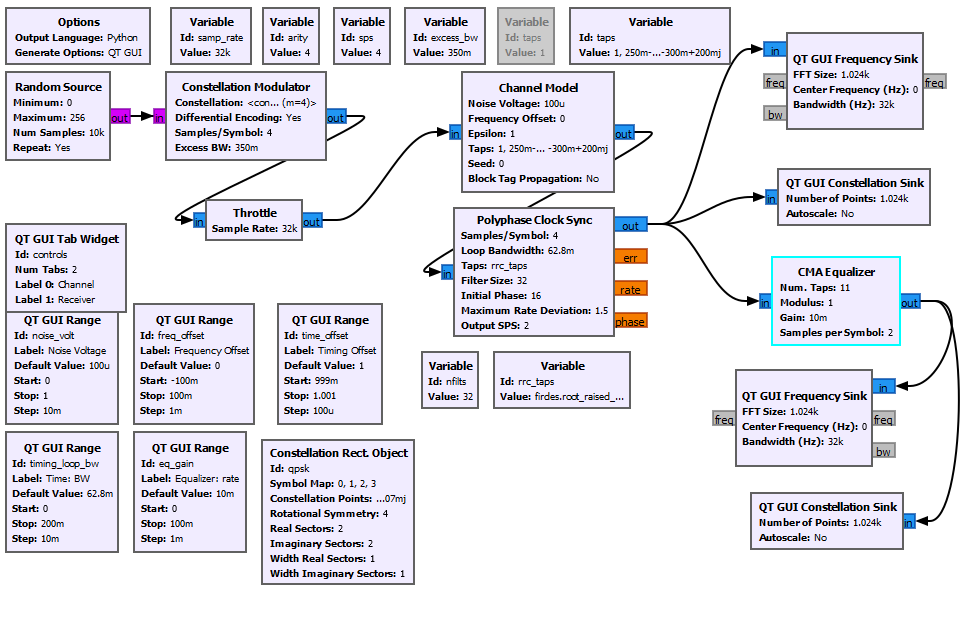
\includegraphics[width=0.8\linewidth]{flowgraph_eq}
        \caption{Flowgraph с эквалайзером CMA}
        \label{fig:flowgraph_eq}
    \end{figure}

    \begin{figure}[H]
        \centering
        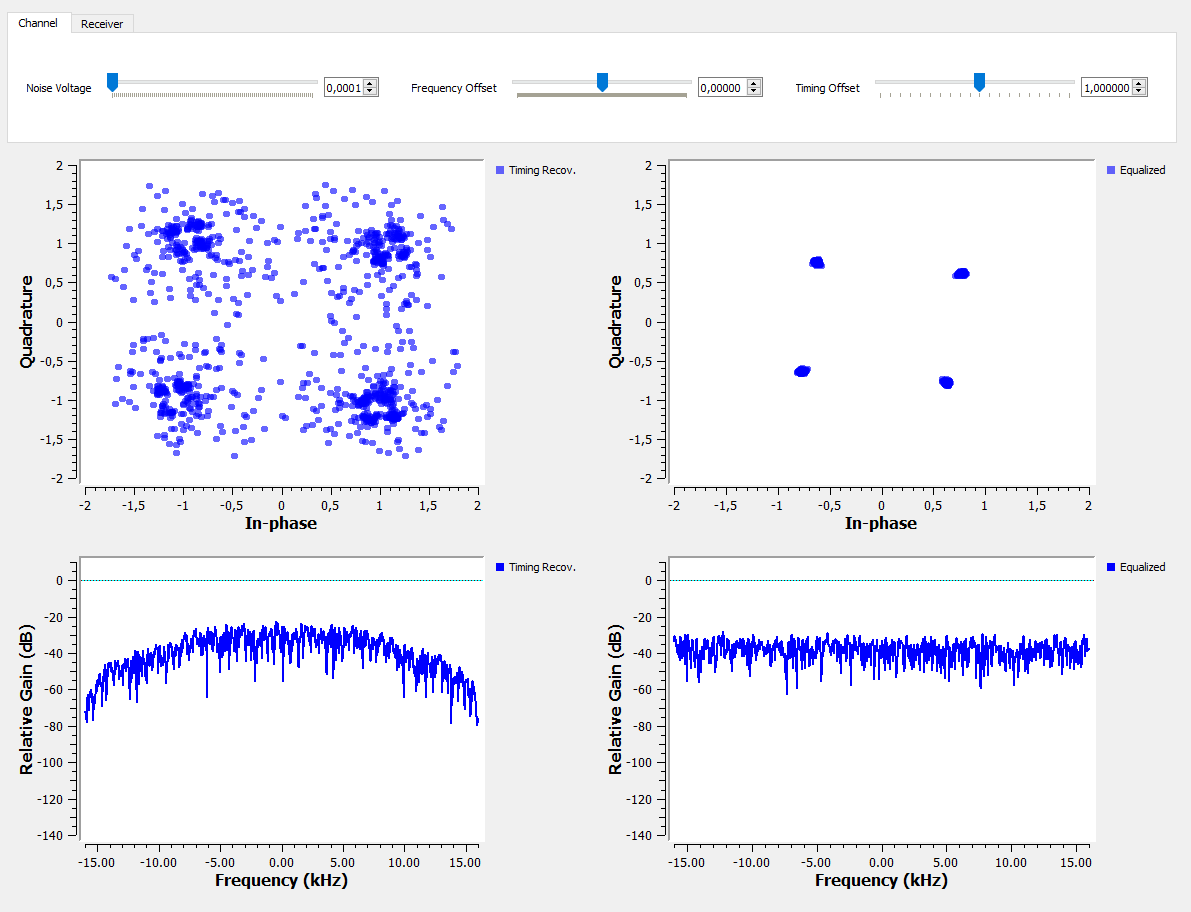
\includegraphics[width=0.8\linewidth]{eq_cma}
        \caption{Использование эквалайзера CMA}
        \label{fig:eq_cma}
    \end{figure}

    На графиках мы можем увидеть эффект синхронизированного по времени многолучевого сигнала до и после эквалайзера.
    До эквалайзера у нас очень некрасивый сигнал даже без шумов.
    Эквалайзер понимает, как инвертировать и сократить канал, чтобы у нас снова был хороший, чистый сигнал.
    Мы также можем видеть сам канал и то, как он красиво выравнивается после эквалайзера.

    \subsection{LMS DD}

    Хорошей практикой является использование блока эквалайзера LMS DD.
    LMS или алгоритм наименьших квадратов требует знания принимаемого сигнала.
    Эквалайзеру необходимо знать точки созвездия для корректировки, и он использует решения о выборках, чтобы сообщить, как обновлять ответвления для эквалайзера.

    Заменим эквалайзер CMA на LMS DD.

    \begin{figure}[H]
        \centering
        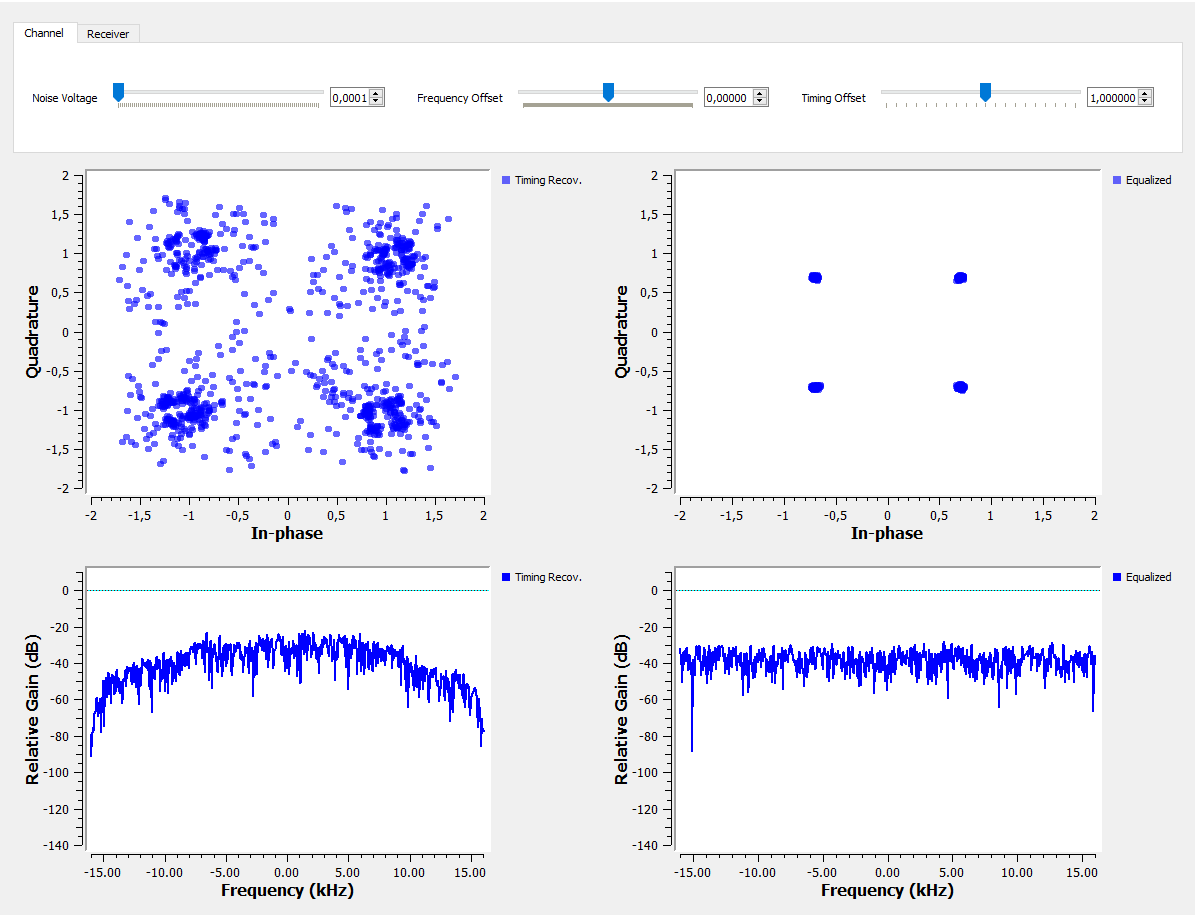
\includegraphics[width=0.8\linewidth]{eq_lms_dd}
        \caption{Использование эквалайзера LMS DD}
        \label{fig:eq_lms_dd}
    \end{figure}

    \newpage


    \section{Фазовая и точная частотная коррекция}
    \label{sec:6}

    Мы выровняли канал, но у нас все еще есть проблема смещения фазы и частоты.
    Она выходит за пределами возможностей эквалайзера.
    Поэтому нам нужно исправить любой сдвиг фазы, а также любой сдвиг частоты.

    На этом этапе мы будем использовать цикл второго порядка, чтобы мы могли отслеживать фазу и частоту.
    Тип восстановления, который мы здесь рассмотрим, предполагает, что мы выполняем точную частотную коррекцию.
    Поэтому мы должны находиться в приличном диапазоне идеальной частоты, чтобы цикл сошёлся.

    Для этой задачи мы собираемся использовать цикл Костаса в примере \texttt{mpsk\_stage5.grc}.

    \begin{figure}[H]
        \centering
        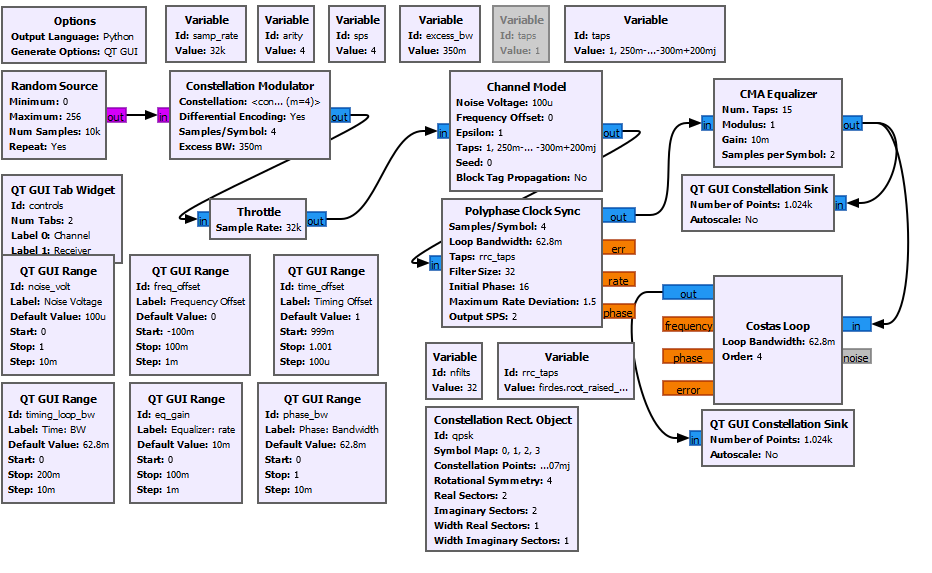
\includegraphics[width=0.8\linewidth]{flowgraph_constas}
        \caption{Flowgraph для исправления сдвига фазы и частоты}
        \label{fig:flowgraph_constas}
    \end{figure}

    \begin{figure}[H]
        \centering
        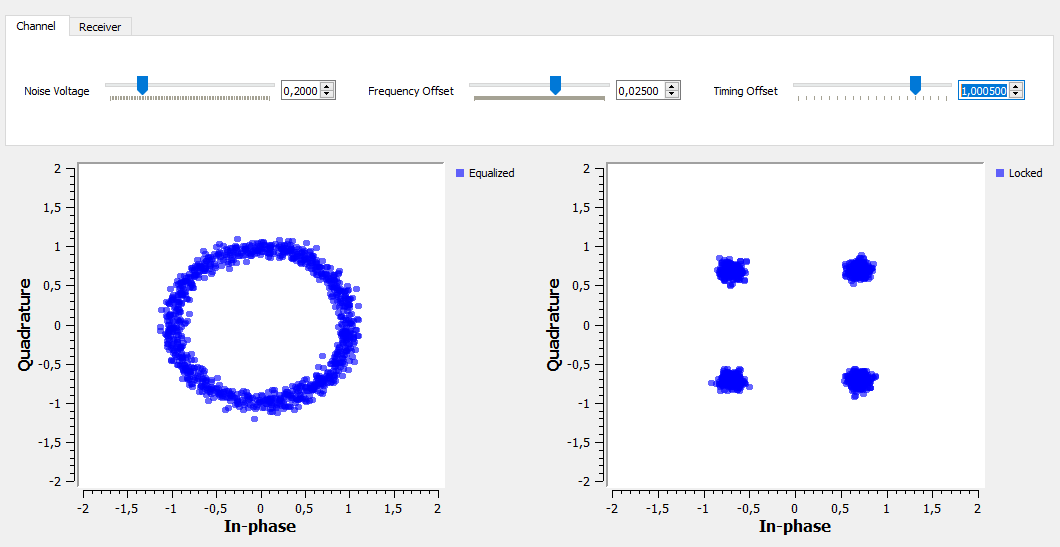
\includegraphics[width=0.8\linewidth]{constas}
        \caption{Исправление сдвига фазы и частоты}
        \label{fig:constas}
    \end{figure}

    Мы установили шум, временной сдвиг, простой многолучевой канал и частотный сдвиг.
    После эквалайзера мы видим, что все символы находятся на единичном круге, но вращаются из-за смещения частоты, которое еще не исправлено.
    На выходе блока цикла Костаса мы можем видеть заблокированное созвездие и дополнительный шум.

    \newpage


    \section{Расшифровка}
    \label{sec:7}

    Теперь мы можем декодировать сигнал.
    Используя пример flowgraph \texttt{mpsk\_stage6.grc}, мы вставляем \texttt{Constellation Decoder} после цикла Костаса, но наша работа еще не завершена.
    Мы передаём 4 дифференциальных символа, но мы не можем быть уверены, что у нас есть такое же отображение символов на точки созвездия, которое мы делали при передаче.

    \begin{figure}[H]
        \centering
        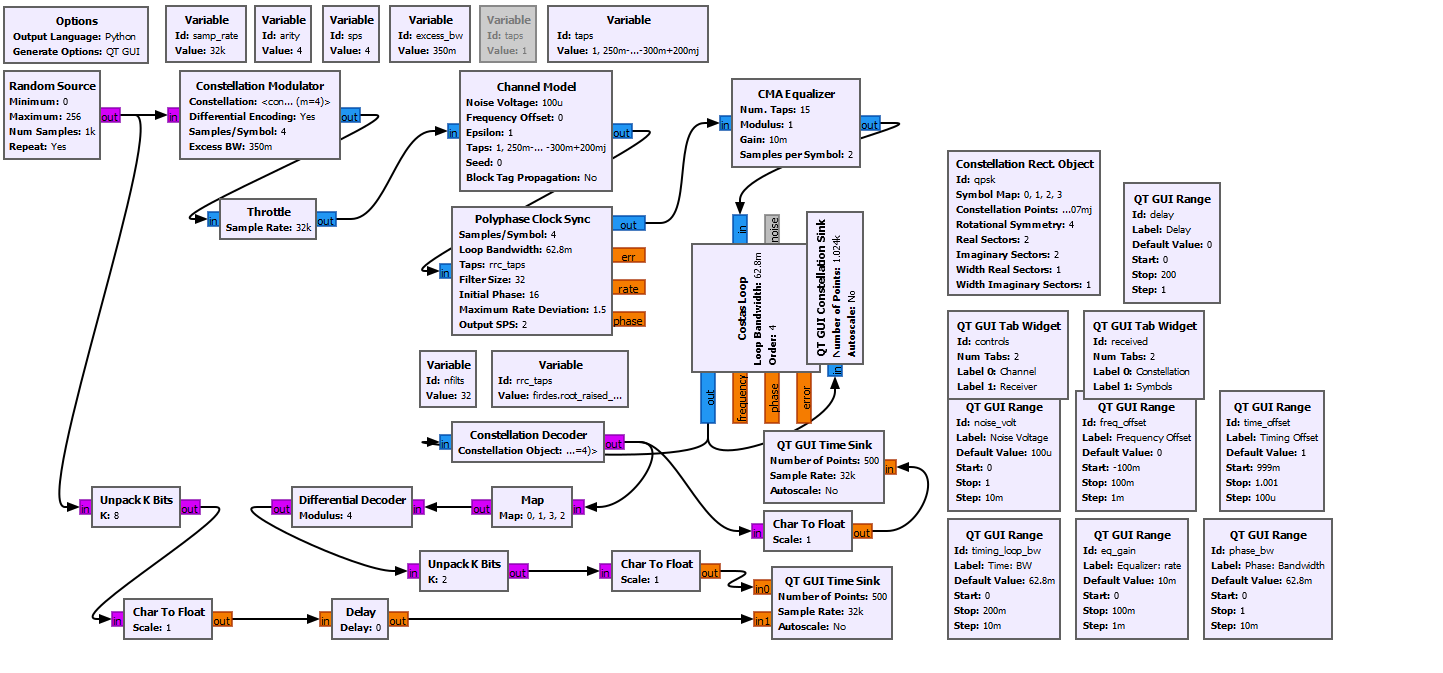
\includegraphics[width=0.8\linewidth]{flowgraph_decoder}
        \caption{Flowgraph декодирования}
        \label{fig:flowgraph_decoder}
    \end{figure}

    Flowgraph использует блок дифференциального декодера для преобразования кодированных дифференциальным кодом символов обратно в их исходные символы.
    Мы используем блок Map для преобразования символов из дифференциального декодера в исходные символы, которые мы передали.
    На данный момент у нас теперь есть исходные символы от 0 до 3, поэтому мы распакуем эти 2 бита на символ в биты, используя блок unpack bits.
    Теперь у нас есть исходный битовый поток данных.

    Но как мы узнаем, что это исходный битовый поток?
    Для этого нам нужно сравнить переданные данные с входным битовым потоком. Однако прямое сравнение ничего не даст.
    Так как в цепочке приемника много блоков и фильтров, которые задерживают сигнал, принятый сигнал отстает на некоторое количество бит.
    Чтобы это исправить, необходимо добавить задержку \texttt{Delay}.

    \begin{figure}[H]
        \centering
        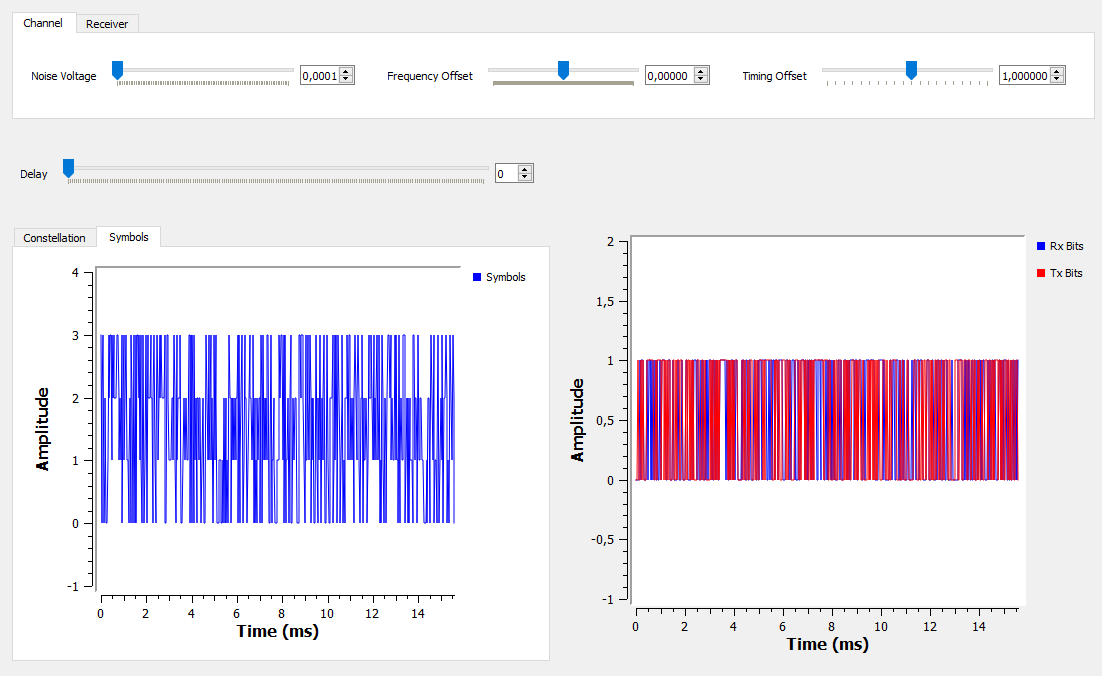
\includegraphics[width=0.8\linewidth]{decoder}
        \caption{Сравнение данных}
        \label{fig:decoder}
    \end{figure}

    \newpage


    \section{Выводы}
    \label{sec:conclusions}

    В результате выполнения данной работы мы изучили основные этапы, необходимые для восстановления сигналов, а также научились строить PSK модулятор/демодулятор для работы с сигналом.

\end{document}